\section{刚性问题}
\label{sec:odenum-stiff}

到目前为止，步长的选择只由精度决定。可是有一类方程，解已经很平缓了，显式方法仍然被迫走极小的步，否则数值解会炸开。先看一个具体的系统。

\paragraph{快速分量追随缓慢分量}
设$x_1$按单位速率衰减，$x_2$以很快的速率追随$x_1$：
\begin{equation}
 \dot{x}_1=-x_1,\qquad \dot{x}_2=50(x_1-x_2),\qquad \bm{x}(0)=\begin{bmatrix}1\\0\end{bmatrix}.
 \label{eq:odenum-stiff-system}
\end{equation}
写成矩阵形式，$\dot{\bm{x}}=\bm{A}\bm{x}$，系数矩阵的特征值是$-1$和$-50$：
\[
 \bm{A}=\begin{bmatrix}-1&0\\50&-50\end{bmatrix}.
\]
线性方程的解法见第~\ref{chap:linear-differential-systems}章，这里直接解出真解：
\begin{equation}
 x_1(t)=\mathrm{e}^{-t},\qquad x_2(t)=\frac{50}{49}\bigl(\mathrm{e}^{-t}-\mathrm{e}^{-50t}\bigr).
 \label{eq:odenum-stiff-exact}
\end{equation}

$\mathrm{e}^{-50t}$一项在$t=0.1$时已经小于$0.7\%$，此后解几乎就是缓慢的$\mathrm{e}^{-t}$（图~\ref{fig:odenum-stiff-scales}）。要描绘这条平缓曲线，步长取$0.1$左右就够了，因为此后真解的时间尺度是$1$。

\begin{BookInlineFigure}
 \centering
 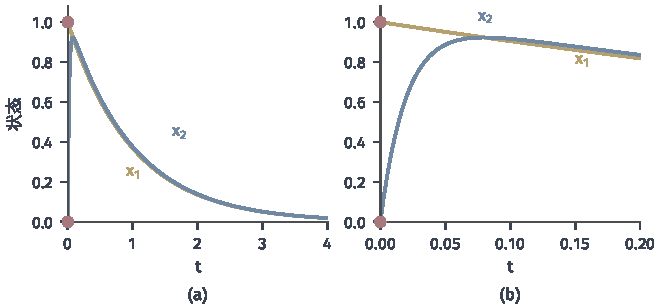
\includegraphics[width=112mm]{figures/06-differential-equations/01-ordinary-differential-equations/matplotlib/odenum-stiff-scales/figure.pdf}
 \caption{系统~\eqref{eq:odenum-stiff-system}的真解，蓝线为$x_2$，黄线为$x_1$，红点是初值。(a)整个区间，两条曲线在初始瞬间之后几乎重合。(b)放大开头的$t\in[0,0.2]$：$x_2$在大约$0.1$的时间内快速追上$x_1$。}
 \label{fig:odenum-stiff-scales}
\end{BookInlineFigure}

\paragraph{显式方法的步长限制}
对这个系统用显式Euler方法。$x_2$的更新是
\[
 x_2^{(k+1)}=(1-50h)\,x_2^{(k)}+50h\,x_1^{(k)}.
\]
括号里的$1-50h$是$x_2$的偏差每步被乘上的因子。$\lvert1-50h\rvert>1$时，偏差逐步放大，真解的平缓与否都救不了它。

取$h=0.05$，因子是$-1.5$，$x_2$的前几步是
\[
 2.5,\quad -1.375,\quad 4.319,\quad -4.335,
\]
而真解在$0.83$到$0.92$之间。取$h=0.03$，因子是$-0.5$，前几步是
\[
 1.5,\quad 0.705,\quad 1.059,\quad 0.840,
\]
逐渐稳定到真解附近（图~\ref{fig:odenum-stiff-euler}）。

\begin{BookInlineFigure}
 \centering
 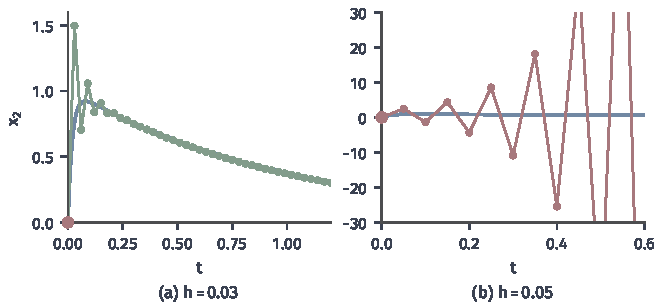
\includegraphics[width=112mm]{figures/06-differential-equations/01-ordinary-differential-equations/matplotlib/odenum-stiff-euler/figure.pdf}
 \caption{显式Euler方法用于系统~\eqref{eq:odenum-stiff-system}的$x_2$分量。蓝线是真解，红点是初值，折线是数值解。(a)$h=0.03$，一步因子$-0.5$，振荡衰减，绿线贴回真解。(b)$h=0.05$，一步因子$-1.5$，红线每步变号并放大。注意两图纵轴的范围不同。}
 \label{fig:odenum-stiff-euler}
\end{BookInlineFigure}

分界在$h=2/50=0.04$。这个限制来自早已衰减殆尽的快速分量，而不是来自要描绘的慢曲线。若把快速率从$50$提高到$5000$，步长上限就成了$4\times10^{-4}$，真解的慢曲线却没有任何变化。

像这样，稳定性对步长的要求比精度的要求严格得多的问题，称为\term{刚性问题}（stiff problem）。刚性没有一个公认的严格定义，它描述的是方程、方法和精度目标三者之间的关系：同一个方程，若目标就是精确刻画开头的快速过程，小步长是精度本身的需要，那就算不上刚性带来的麻烦。

第~\ref{sec:odenum-error-convergence}节的误差界在这里帮不上忙。系统的Lipschitz常数大约是$50$，定理~\ref{thm:odenum-global-error}的放大因子$\mathrm{e}^{\Lambda T}$在$T=4$时是$\mathrm{e}^{200}$量级。Lipschitz常数只看变化率的大小，看不出快速模式是在衰减还是在增长，所以需要另一种分析。

\subsection{绝对稳定性}
\label{sec:odenum-absolute-stability}

固定步长$h$，让步数不断增加，数值解中的扰动是衰减还是放大？回答这个问题的标准工具是一个最简单的方程。

\paragraph{测试方程与放大因子}
取标量线性方程，$\lambda$允许为复数，复数$\lambda$对应振荡的模式：
\begin{equation}
 \dot{x}=\lambda x,\qquad \lambda\in\mathbb{C}.
 \label{eq:odenum-test-equation}
\end{equation}
它称为\term{测试方程}（test equation）。对这个方程，一步方法每步把数值解乘上一个只依赖$z=h\lambda$的数$R(z)$，$R$称为方法的\term{放大因子}（amplification factor），也叫稳定函数。

逐个方法代入。显式Euler方法给出
\[
 x^{(k+1)}=x^{(k)}+h\lambda x^{(k)},
\]
所以$R(z)=1+z$。

中点方法的两个斜率分别是
\[
 k_1=\lambda x^{(k)},\qquad k_2=\lambda\Bigl(1+\frac{z}{2}\Bigr)x^{(k)},
\]
代入更新式$x^{(k+1)}=x^{(k)}+hk_2$，得到
\[
 R(z)=1+z+\frac{z^2}{2}.
\]

RK4的四个斜率依次为
\[
 \begin{aligned}
  k_1&=\lambda x^{(k)},\\
  k_2&=\lambda\Bigl(1+\frac{z}{2}\Bigr)x^{(k)},\\
  k_3&=\lambda\Bigl(1+\frac{z}{2}+\frac{z^2}{4}\Bigr)x^{(k)},\\
  k_4&=\lambda\Bigl(1+z+\frac{z^2}{2}+\frac{z^3}{4}\Bigr)x^{(k)}.
 \end{aligned}
\]
代入$\tfrac{h}{6}(k_1+2k_2+2k_3+k_4)$并合并同类项，得到
\[
 R(z)=1+z+\frac{z^2}{2}+\frac{z^3}{6}+\frac{z^4}{24}.
\]

三个放大因子都是$\mathrm{e}^{z}$的Taylor截断，截断的次数恰好等于方法的阶。真解每步被乘$\mathrm{e}^{z}$，$R(z)$就是对它的近似。

\begin{definition}[绝对稳定域]
 \label{def:odenum-stability-region}
 一步方法用于测试方程~\eqref{eq:odenum-test-equation}时若满足$x^{(k+1)}=R(z)x^{(k)}$，称
 \begin{equation}
  \bm{S}=\bigl\{z\in\mathbb{C}:\lvert R(z)\rvert\leq1\bigr\}
  \label{eq:odenum-stability-region}
 \end{equation}
 为方法的\term{绝对稳定域}（region of absolute stability）。
\end{definition}

当$\mathrm{Re}\,\lambda<0$时，测试方程的真解衰减，$\lvert\mathrm{e}^{z}\rvert<1$。我们希望数值解也不放大，这就要求$h\lambda$落在稳定域内。

\paragraph{从测试方程到线性系统}
为什么一个标量方程能说明系统的问题？设$\bm{A}$可对角化，$\bm{A}=\bm{V}\bm{D}\bm{V}^{-1}$。令$\bm{w}=\bm{V}^{-1}\bm{x}$，对显式Euler方法，
\[
 \bm{w}^{(k+1)}=(\bm{I}+h\bm{D})\bm{w}^{(k)},
\]
每个模式各自按测试方程演化。其他Runge--Kutta方法同样如此，因为它们都只用$\bm{A}$的多项式。

于是数值解不放大的条件是每个$h\lambda_i$都落在$\bm{S}$中。对系统~\eqref{eq:odenum-stiff-system}，$\lambda=-1$给出$z=-h$，$\lambda=-50$给出$z=-50h$；后者的约束才是起作用的。

\paragraph{稳定域的形状}
图~\ref{fig:odenum-stability-explicit}画出三个显式方法的稳定域。显式Euler方法的稳定域是以$-1$为心的单位圆盘，在负实轴上止于$-2$，这就是步长限制$h\leq2/\lvert\lambda\rvert$的来源。图中红点$z=-2.5$对应$h=0.05$，绿点$z=-1.5$对应$h=0.03$，与上面的计算一致。

\begin{BookInlineFigure}
 \centering
 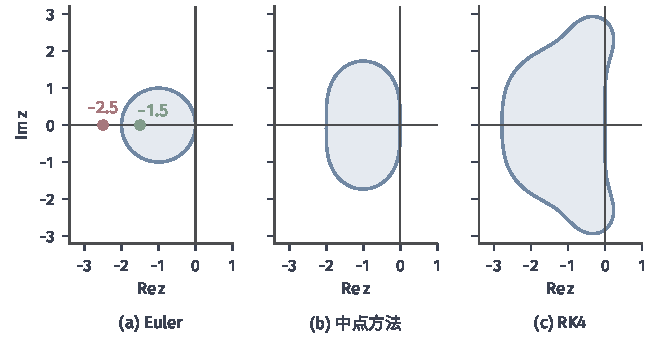
\includegraphics[width=112mm]{figures/06-differential-equations/01-ordinary-differential-equations/matplotlib/odenum-stability-explicit/figure.pdf}
 \caption{显式方法的绝对稳定域（浅蓝），边界是$\lvert R(z)\rvert=1$，三幅图的坐标范围相同。(a)显式Euler方法，红点$z=-2.5$在域外，绿点$z=-1.5$在域内；(b)中点方法，实轴上止于$-2$；(c)RK4，实轴上止于约$-2.785$。}
 \label{fig:odenum-stability-explicit}
\end{BookInlineFigure}

阶数提高，稳定域略有扩大，但RK4的实轴范围也只到约$-2.785$。原因在结构上：显式Runge--Kutta方法的$R(z)$总是多项式，当$\lvert z\rvert\to\infty$时$\lvert R(z)\rvert\to\infty$，所以稳定域必定有界。高阶的显式方法解除不了刚性带来的限制。

\paragraph{这一分析能说明什么}
测试方程分析的是数值扰动怎样传播，适用的情形是线性、常系数、矩阵可对角化，并且步长固定。在非线性问题上，通常把$\partial_{\bm{x}}\bm{f}$沿解冻结在某一时刻来做估计，这只是启发式的做法。它不能代替第~\ref{sec:odenum-error-convergence}节那样的收敛论证。

下面的时变系统说明冻结的特征值可能误导人。取矩阵
\[
 \bm{A}(t)=\begin{bmatrix}
  -1+\tfrac{3}{2}\cos^2t & 1-\tfrac{3}{2}\sin t\cos t\\
  -1-\tfrac{3}{2}\sin t\cos t & -1+\tfrac{3}{2}\sin^2t
 \end{bmatrix}.
\]
它的迹恒为$-1/2$，行列式恒为$1/2$，所以每个时刻的特征值都是$(-1\pm\mathrm{i}\sqrt{7})/4$，实部为$-1/4$，全在左半平面。

可是直接代入可以验证，下面的函数是方程$\dot{\bm{x}}=\bm{A}(t)\bm{x}$的解：
\[
 \bm{x}(t)=\mathrm{e}^{t/2}\begin{bmatrix}\cos t\\-\sin t\end{bmatrix},
\]
它的长度按$\mathrm{e}^{t/2}$增长（图~\ref{fig:odenum-frozen-coefficients}）。每一时刻看起来都是衰减的，解却在增长，因为特征方向在随时间转动。

\begin{BookInlineFigure}
 \centering
 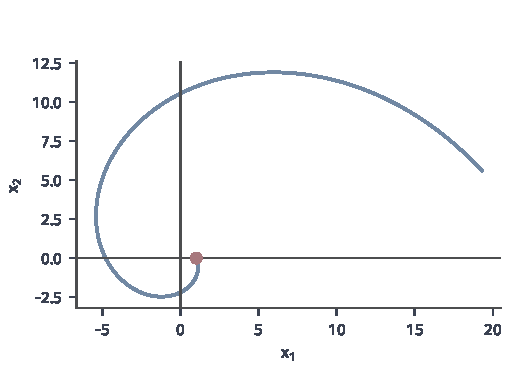
\includegraphics[width=86mm]{figures/06-differential-equations/01-ordinary-differential-equations/matplotlib/odenum-frozen-coefficients/figure.pdf}
 \caption{冻结特征值全在左半平面的时变线性系统。蓝线是从红点$(1,0)$出发的解，在$t\in[0,6]$上按$\mathrm{e}^{t/2}$向外旋转。}
 \label{fig:odenum-frozen-coefficients}
\end{BookInlineFigure}

\begin{BookInlineTable}
 \centering
 \caption{收敛与绝对稳定性的对比。}
 \label{tab:odenum-convergence-stability}
 \begin{tabular}{lll}
  \toprule
  & 收敛（定理~\ref{thm:odenum-global-error}） & 绝对稳定性\\
  \midrule
  关心的极限 & 固定$T$，$h\to0$ & 固定$h$，步数增加\\
  适用问题 & 非线性，有限区间 & 线性测试方程\\
  回答的问题 & 误差怎样随$h$减小 & 扰动是否放大\\
  \bottomrule
 \end{tabular}
\end{BookInlineTable}

\subsection{隐式格式}
\label{sec:odenum-implicit}

显式方法的放大因子是多项式，稳定域有界。要让稳定域覆盖整个左半平面，$R(z)$必须换成有理函数，这要求更新式的右端用到未知的新值。

\paragraph{主要思想}
回到积分式~\eqref{eq:odenum-integral-step}。Euler方法用左端点的值近似被积函数，现在改用右端点的值，得到\term{后向Euler方法}（backward Euler method）：
\begin{equation}
 \bm{x}^{(k+1)}=\bm{x}^{(k)}+h\,\bm{f}\bigl(t_{k+1},\bm{x}^{(k+1)}\bigr).
 \label{eq:odenum-backward-euler}
\end{equation}
未知的$\bm{x}^{(k+1)}$出现在等式两边，每一步都要解一个方程，这样的方法称为\term{隐式方法}（implicit method）。

把左右两端点的值平均，得到\term{梯形方法}（trapezoidal rule）：
\begin{equation}
 \bm{x}^{(k+1)}=\bm{x}^{(k)}+\frac{h}{2}\Bigl(\bm{f}\bigl(t_k,\bm{x}^{(k)}\bigr)+\bm{f}\bigl(t_{k+1},\bm{x}^{(k+1)}\bigr)\Bigr).
 \label{eq:odenum-trapezoid}
\end{equation}

在非刚性问题上它们的局部误差可以直接估计。对后向Euler方法，设$\bm{x}\in C^2$，$hL<1$，$\bm{y}=\bm{\Psi}_h(t_k,\bm{x}(t_k))$。真解满足同一个方程，只多一个余项$\bm{r}$，其大小满足
\[
 \lVert\bm{r}\rVert_2\leq\frac{h^2}{2}\max_{t}\lVert\ddot{\bm{x}}(t)\rVert_2.
\]
两式相减得到
\[
 \lVert\bm{y}-\bm{x}(t_{k+1})\rVert_2\leq hL\lVert\bm{y}-\bm{x}(t_{k+1})\rVert_2+\lVert\bm{r}\rVert_2,
\]
移项得到
\[
 \bigl\lVert\bm{\ell}^{(k+1)}\bigr\rVert_2\leq\frac{\lVert\bm{r}\rVert_2}{1-hL},
\]
所以后向Euler方法的阶是$1$。

梯形方法的阶是$2$，要求$\bm{x}\in C^3$：梯形求积公式的余项是$O(h^3)$，推导方式相同。这里的估计用了$hL<1$，刚性问题的$hL$很大，上面的估计就失去了意义，要靠下面的稳定性分析。

\paragraph{放大因子与稳定域}
把后向Euler方法用于测试方程，得到$x^{(k+1)}=x^{(k)}+zx^{(k+1)}$，解出
\begin{equation}
 R(z)=\frac{1}{1-z}.
 \label{eq:odenum-be-factor}
\end{equation}
于是$\lvert R(z)\rvert\leq1$等价于$\lvert1-z\rvert\geq1$，稳定域是以$1$为心的单位开圆盘的外部。

对梯形方法，同样的计算给出
\begin{equation}
 R(z)=\frac{1+z/2}{1-z/2}.
 \label{eq:odenum-trapezoid-factor}
\end{equation}
直接展开两个模的平方可得
\[
 \lvert1+z/2\rvert^2-\lvert1-z/2\rvert^2=2\,\mathrm{Re}\,z,
\]
所以$\lvert R(z)\rvert\leq1$恰好等价于$\mathrm{Re}\,z\leq0$，稳定域就是闭左半平面（图~\ref{fig:odenum-stability-implicit}）。

\begin{BookInlineFigure}
 \centering
 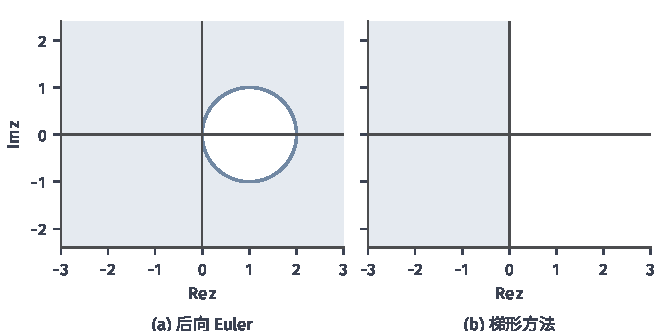
\includegraphics[width=112mm]{figures/06-differential-equations/01-ordinary-differential-equations/matplotlib/odenum-stability-implicit/figure.pdf}
 \caption{隐式方法的绝对稳定域（浅蓝）。(a)后向Euler方法，稳定域是以$1$为心的单位开圆盘（白色）的外部；(b)梯形方法，稳定域恰为闭左半平面。两者都包含闭左半平面，图中只画出有限范围。}
 \label{fig:odenum-stability-implicit}
\end{BookInlineFigure}

若稳定域包含闭左半平面，就称方法\term{A稳定}（A-stable）。这两个隐式方法都是A稳定的，因此用于系统~\eqref{eq:odenum-stiff-system}时不论$h$多大，线性模式都不会被放大。

\paragraph{快速模式的数值阻尼}
A稳定只保证不放大，不保证快速模式被迅速消除。比较$z\to-\infty$时的极限：真解的因子$\mathrm{e}^{z}\to0$，后向Euler的$R(z)\to0$，梯形方法的$R(z)\to-1$（图~\ref{fig:odenum-amplification-real}）。

\begin{BookInlineFigure}
 \centering
 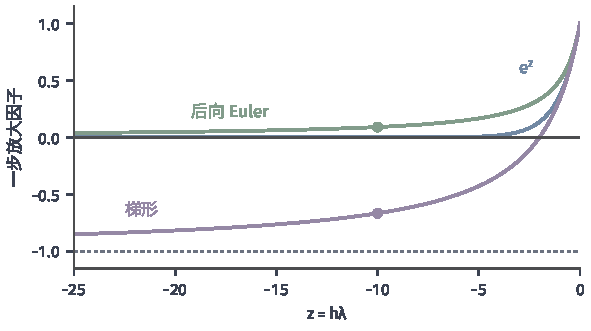
\includegraphics[width=100mm]{figures/06-differential-equations/01-ordinary-differential-equations/matplotlib/odenum-amplification-real/figure.pdf}
 \caption{负实轴上的一步放大因子。蓝线是真解的$\mathrm{e}^{z}$，绿线是后向Euler的$1/(1-z)$，紫线是梯形方法的$(1+z/2)/(1-z/2)$，灰色虚线是$-1$。圆点标出$z=-10$处的取值$1/11$和$-2/3$。}
 \label{fig:odenum-amplification-real}
\end{BookInlineFigure}

后向Euler对快速模式有很强的\term{数值阻尼}（numerical damping），模式一步就几乎消失。梯形方法的快速模式几乎不衰减，只是每步变号。在$z=-10$时，后向Euler的因子是$1/11$，梯形方法是$-2/3$。若方法既A稳定又满足$\lim_{z\to-\infty}R(z)=0$，就称方法\term{L稳定}（L-stable），后向Euler是，梯形方法不是。

\paragraph{计算过程：线性系统}
线性系统$\dot{\bm{x}}=\bm{A}\bm{x}$上，后向Euler方法每步解一个线性方程组，结果可以写成显式形式：
\begin{equation}
 \bm{x}^{(k+1)}=(\bm{I}-h\bm{A})^{-1}\bm{x}^{(k)}.
 \label{eq:odenum-be-linear}
\end{equation}
实际计算不求逆，而是分解一次$\bm{I}-h\bm{A}$再反复回代，步长不变时每步只需回代。下面用系统~\eqref{eq:odenum-stiff-system}演示，取$h=0.2$，它是显式方法上限$0.04$的五倍。

\needspace{6\baselineskip}
\paragraph{变量}
\begin{itemize}
 \item $\bm{x}^{(k)}\in\mathbb{R}^{n}$：第$k$个网格点的数值解。
 \item $\bm{I}-h\bm{A}\in\mathbb{R}^{n\times n}$：每步的系数矩阵，步长不变时只分解一次。
\end{itemize}

\paragraph{初始化}
把数值解初始化为初值，并构造系数矩阵。例中
\[
 \bm{x}^{(0)}=\begin{bmatrix}1\\0\end{bmatrix},\qquad
 \bm{I}-h\bm{A}=\begin{bmatrix}1.2&0\\-10&11\end{bmatrix}.
\]

\needspace{6\baselineskip}
\paragraph{每轮更新}
对$k=0,1,\ldots,N-1$依次执行：
\begin{enumerate}
 \item \textbf{求解第一个分量。}例中系数矩阵是下三角的，由第一行得到
 \[
  x_1^{(k+1)}=\frac{x_1^{(k)}}{1+h}.
 \]
 例中第一轮
 \[
  x_1^{(1)}=\frac{1}{1.2}=0.833333.
 \]
 \item \textbf{求解第二个分量。}由第二行得到
 \[
  x_2^{(k+1)}=\frac{x_2^{(k)}+50h\,x_1^{(k+1)}}{1+50h}.
 \]
 例中第一轮
 \[
  x_2^{(1)}=\frac{0+10\times0.833333}{11}=0.757576.
 \]
 例中第二轮，两个分量依次为
 \[
  x_1^{(2)}=0.694444,\qquad x_2^{(2)}=\frac{0.757576+6.944444}{11}=0.700184.
 \]
 \item \textbf{停止。}走满$N$步后结束。
\end{enumerate}
最终例中$t=0.4$处$x_2^{(2)}=0.700184$，真值约为$0.684000$，没有振荡。第一步的误差较大，因为$h=0.2$完全跨过了快速过渡，这是用一步盖过快速过程的代价，后面的步很快贴回真解。

图~\ref{fig:odenum-implicit-stiff}比较两种隐式方法。梯形方法的第一轮为
\[
 x_2^{(1)}=\frac{5\,(x_1^{(0)}+x_1^{(1)})-4\,x_2^{(0)}}{6}=1.515152,
\]
其中$x_1^{(1)}=0.818182$。它明显越过真解，之后按因子$-2/3$交替变号衰减，正好体现了图~\ref{fig:odenum-amplification-real}中$z=-10$处的差别。

\begin{BookInlineFigure}
 \centering
 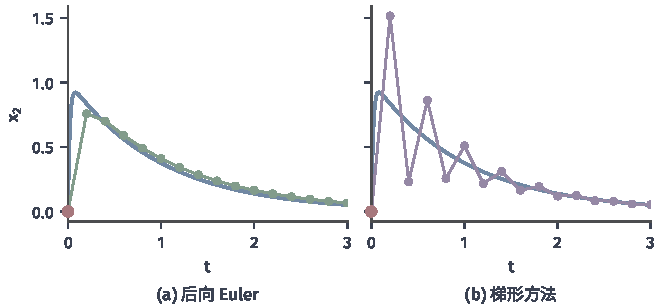
\includegraphics[width=112mm]{figures/06-differential-equations/01-ordinary-differential-equations/matplotlib/odenum-implicit-stiff/figure.pdf}
 \caption{隐式方法用于系统~\eqref{eq:odenum-stiff-system}，$h=0.2$，纵轴为$x_2$。蓝线是真解，红点是初值。(a)后向Euler方法（绿）没有振荡；(b)梯形方法（紫）第一步越过真解，之后交替变号衰减。}
 \label{fig:odenum-implicit-stiff}
\end{BookInlineFigure}

\paragraph{计算过程：非线性方程}
非线性问题的隐式更新没有闭式，需要迭代。对后向Euler方法，设$\bm{y}$是要求的$\bm{x}^{(k+1)}$，解方程
\begin{equation}
 \bm{G}(\bm{y})=\bm{y}-\bm{x}^{(k)}-h\,\bm{f}(t_{k+1},\bm{y})=\bm{0}.
 \label{eq:odenum-implicit-equation}
\end{equation}

最直接的不动点迭代$\bm{y}\leftarrow\bm{x}^{(k)}+h\bm{f}(t_{k+1},\bm{y})$只在$hL<1$时保证压缩，这恰好是显式方法的步长量级，隐式方法的好处就丢掉了。所以刚性问题通常用Newton迭代，即每次解线性方程组
\[
 \bigl(\bm{I}-h\,\partial_{\bm{x}}\bm{f}(t_{k+1},\bm{y})\bigr)\bm{\Delta}=-\bm{G}(\bm{y}),
\]
再令$\bm{y}\leftarrow\bm{y}+\bm{\Delta}$。Newton法的收敛性质可参考\BookChapterRef{chap:second-order-methods}{卷五第7章“二阶方法”}，线性方程组的分解可参考\BookChapterRef{chap:direct-linear-solvers}{卷二第12章“线性方程的直接求解”}。

用例~\eqref{eq:odenum-running}演示，$h=0.5$。一维时
\[
 G(y)=y-x^{(k)}-0.5\,y(1-y),\qquad G'(y)=1-0.5(1-2y).
\]
以显式Euler的结果$y=0.28$作初值，第一步的迭代为
\[
 G(0.28)=-0.0208,\quad G'(0.28)=0.78,\quad y=0.306667.
\]
第二次迭代得到
\[
 G(0.306667)=3.56\times10^{-4},\quad G'(0.306667)=0.806667,\quad y=0.306226.
\]
此时$\lvert G\rvert$已降到$10^{-7}$量级，取$x^{(1)}=0.306226$。

\paragraph{内部容差计入误差预算}
隐式更新解不到严格的零。迭代提前停止留下的偏差，正是式~\eqref{eq:odenum-computed}中的计算误差$\bm{\delta}^{(k+1)}$。由定理~\ref{thm:odenum-global-error}，它在全局误差中贡献$\varepsilon/h$的量级。

图~\ref{fig:odenum-inner-tolerance}给出一个实验：对例~\eqref{eq:odenum-running}用梯形方法，内部用不动点迭代（此处$h$较小，迭代是压缩的），当相邻两次迭代之差不超过内部容差时停止。容差很小时，误差停在由截断决定的平台；容差放松到一定程度，误差会阶梯式上升，最宽松时一次迭代就停，格式退化为一阶。

\begin{BookInlineFigure}
 \centering
 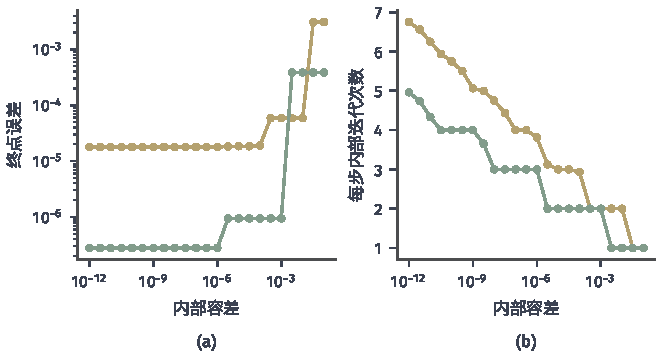
\includegraphics[width=112mm]{figures/06-differential-equations/01-ordinary-differential-equations/matplotlib/odenum-inner-tolerance/figure.pdf}
 \caption{内部方程的容差对梯形方法的影响，问题为式~\eqref{eq:odenum-running}，$T=1$，内部采用不动点迭代。黄线$N=16$，绿线$N=128$。(a)终点误差：容差小时不随容差变化，容差大时误差阶梯式上升。(b)每步平均内部迭代次数：容差越小迭代越多。}
 \label{fig:odenum-inner-tolerance}
\end{BookInlineFigure}

这个实验给出的预算原则是：内部容差要明显小于这一步允许的局部误差，否则花在高阶公式上的计算会被内部误差抵消；反过来把容差压得远低于截断误差，只是白白增加迭代次数。

\paragraph{不能只看阶数}
选择方法时要同时考虑稳定域、每步求解代价和计算误差。对系统~\eqref{eq:odenum-stiff-system}，RK4虽然是四阶，步长仍受$2.785/50\approx0.056$的限制，走到$T=4$至少$72$步、$288$次右端求值。一阶的后向Euler方法取$h=0.2$只需$20$步，每步解一次$2\times2$的线性方程组，而且不会发散。

反过来，方程若不刚性，隐式方法每步要解方程，就比显式方法贵得多，也得不到额外好处。表~\ref{tab:odenum-implicit-compare}汇总本节的方法。

\begin{BookInlineTable}
 \centering
 \caption{显式与隐式方法的对比，$z=h\lambda$。}
 \label{tab:odenum-implicit-compare}
 \begin{tabular}{llcc}
  \toprule
  方法 & $R(z)$ & 阶 & A稳定\\
  \midrule
  显式Euler & $1+z$ & 1 & 否\\
  RK4 & 四次多项式 & 4 & 否\\
  后向Euler & $1/(1-z)$ & 1 & 是，$R(-\infty)=0$\\
  梯形 & $(1+z/2)/(1-z/2)$ & 2 & 是，$R(-\infty)=-1$\\
  \bottomrule
 \end{tabular}
\end{BookInlineTable}

